\section{Feasibility and Scope}

\subsection{Target Audience}
\begin{frame}{Target Audience}
	The project aims to target the following audiences:
	\begin{enumerate}
		\item Online shoppers
		\item Fashion enthusiasts and bloggers
		\item Busy professionals
		\item E-commerce retailers
		\item Fashion brands
	\end{enumerate}
\end{frame}

\subsection{Feasibility}
\begin{frame}[allowframebreaks]{Feasibility}
	\begin{itemize}
		\item \textbf{Legal Feasibility:}
			\begin{itemize}
				\item High-quality ethically-sourced datasets are publically available for use.
				\item Data privacy and security can be ensured by collecting minimum data as per user consent.
			\end{itemize}
		\item \textbf{Technical Feasibility:}
			\begin{itemize}
				\item Personalized recommendation systems can be built using techniques like Matrix Factorization and Bayesian Personalized Ranking.
				\item Intermediary tasks can be handled using embeddings and feature extraction techniques.
				\item Even simple mobile cameras have already been used to cast clothes on human body shapes.
			\end{itemize}
		\item \textbf{Scheduling Feasibility:} The project can be successfully completed within the term.
		
		\pagebreak

		\item \textbf{Economic Feasibility:}
			\begin{itemize}
				\item Model training can be done on consumer-grade hardware in addition to services like Google Colab, or Runpod which provides low-cost Cloud GPUs \cite{runpodInstancePricing}:
				\begin{table}
					\vspace*{0.25cm}
					\centering
					\begin{tabular}{c|c|c|c|c}
						\textbf{VRAM (GB)} & 20 & 24 & 48 & 80 \\
						\hline
						\textbf{$\sim$INR/hr} & 30 & 35 & 63 & 166 \\
					\end{tabular}
					\vspace*{0.25cm}
				\end{table}
				\item Inference can be done on consumer-grade hardware without needing extra purchases.
			\end{itemize}

		\item \textbf{Operational Feasibility:} A user-friendly interface which accomplishes the objectives of the project with ease of maintenance and integration of future work can be developed.
	\end{itemize}
\end{frame}

\subsection{Scope}
\begin{frame}{Scope}
	The project has the following scope:
	\begin{enumerate}
		\item \textbf{Fashion embedding:} Embed clothing items in higher-dimensional space.
		\item \textbf{Feature extractor:} Train feature extractor for body part segmentation.
		\item \textbf{AI-based recommender:} Train a personalized recommendation system.
		\item \textbf{AR virtual try-on:} Develop an AR-powered virtual try-on module.
	\end{enumerate}
\end{frame}

\subsection{Timeline Diagram}
\begin{frame}{Timeline Diagram}
	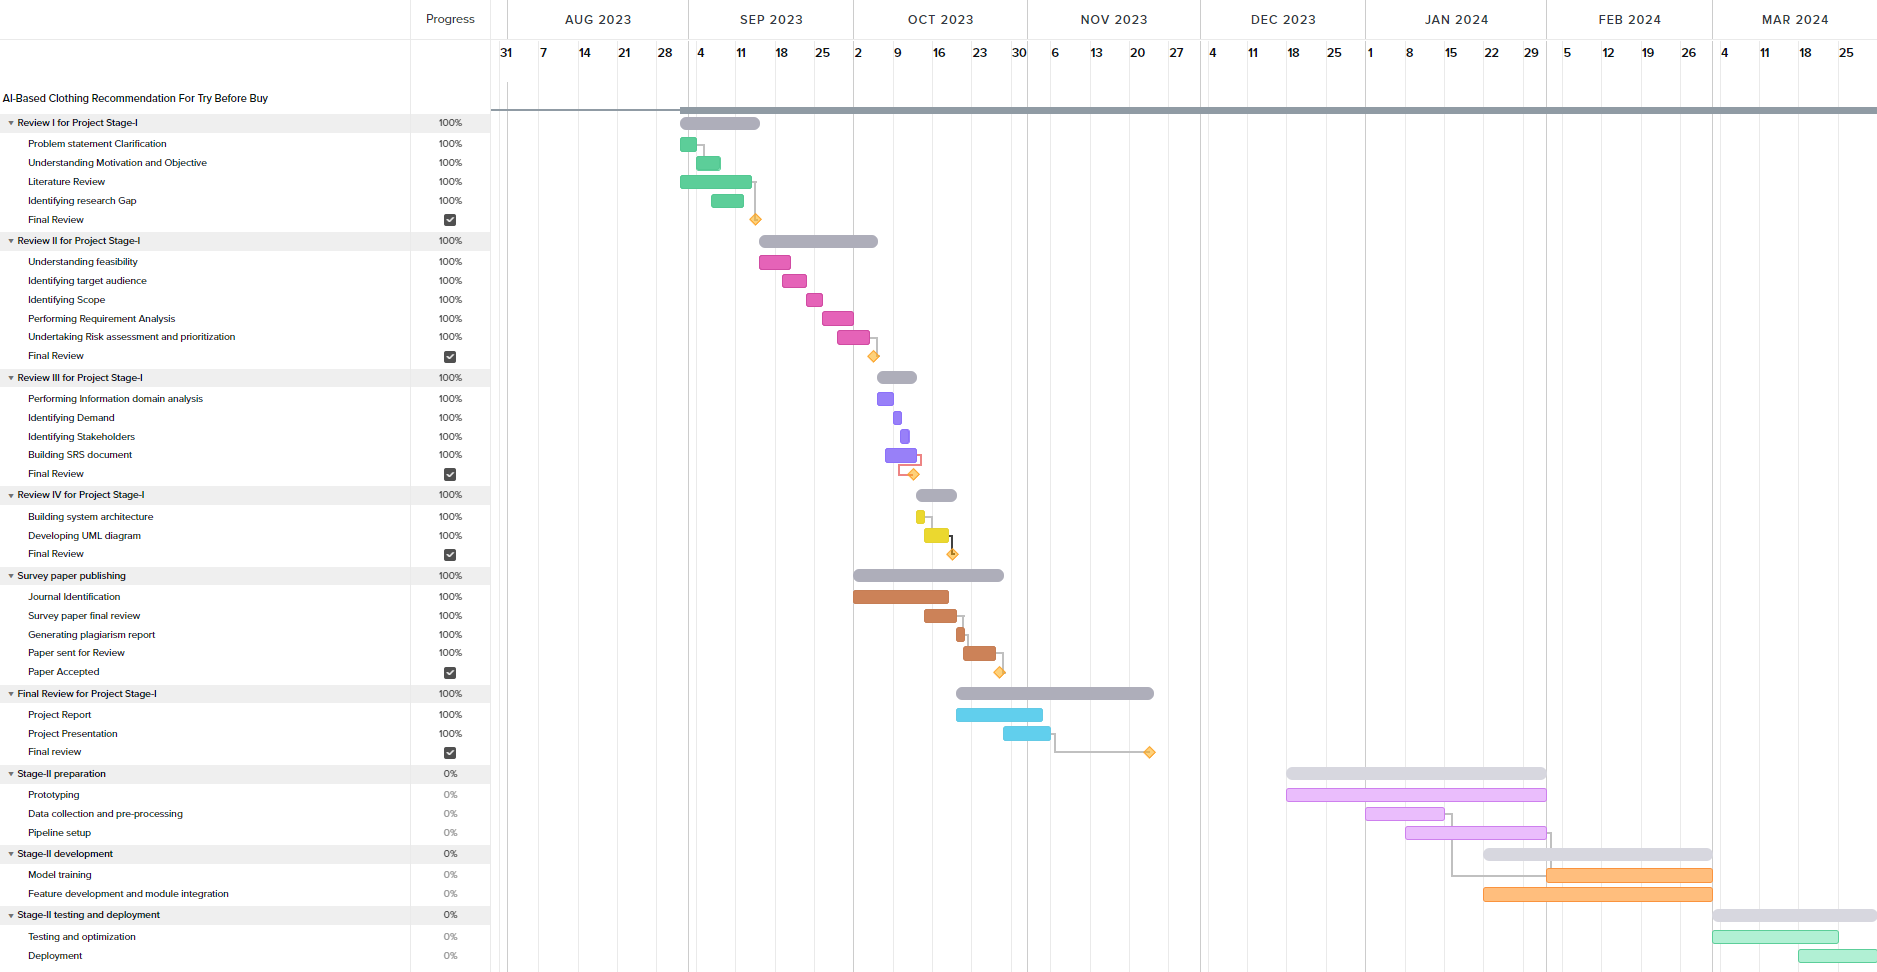
\includegraphics[width=\textwidth]{components/images/timeline.png}
\end{frame}

\subsection{Risk Assessment}
\begin{frame}{Risk Assessment}
	The following risks were identified with the project:
	\begin{enumerate}
		\item Removal of existing garments from the subject.
		\item Inappropriate recommendations for certain age groups or gender classes.
		\item Bias towards certain gender, body shape, size, skin color, etc.
	\end{enumerate}
	These can be mitigated by rigorous testing and implementing multiple failsafes.
\end{frame}
